% Inbuilt themes in beamer
\documentclass{beamer}

% Theme choice:
\usetheme{Madrid}
\usepackage{empheq}
\usefonttheme[onlymath]{serif}
% Title page details: 
\title{Vibration-Rotation in Many Dimensions} 
\author{Yunting-Bu}
\date{\today}
\logo{\large \LaTeX{}}


\begin{document}
	% Title page frame
	\begin{frame}
		\titlepage 
	\end{frame}
	
	% Remove logo from the next slides
	\logo{}
	% Outline frame
	\begin{frame}{Outline}
		\tableofcontents
	\end{frame}
	% Lists frame
	\section{Triatomic Molecules}
	\begin{frame}{Triatomic Molecules}
		For a triatomic molecule, there are total of three sets of Jacobi coordinates.
		\begin{figure}[H]
			\centering
			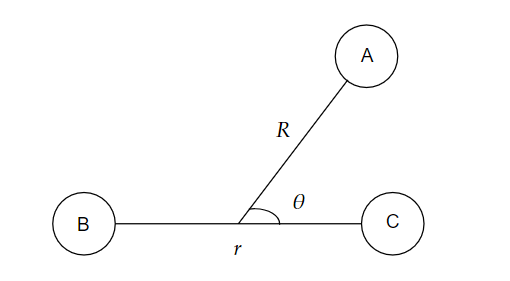
\includegraphics[scale=0.5]{1.png}
			\caption{Jacobi coordinates}
			\label{Figure1}
		\end{figure}
	\end{frame}
	\begin{frame}{Triatomic Molecules}
		The kinetic energy operator is diagonal, and the triatomic Hamiltonian is given by the following
		\begin{align}
			H&=-\dfrac{\hbar^2}{2\mu_R}\nabla^2_R-\dfrac{\hbar^2}{2\mu_r}\nabla^2_r+V(\mathbf{R},\mathbf{r})\nonumber\\
			&=\dfrac{\hbar^2}{2\mu_R}\dfrac{1}{R}\dfrac{\partial^2}{\partial R^2}R+\dfrac{\mathbf{L}^2}{2\mu_RR^2}-\dfrac{\hbar^2}{2\mu_r}\dfrac{1}{r}\dfrac{\partial^2}{\partial r^2}r+\dfrac{\mathbf{j}^2}{2\mu_rr^2}+V(\mathbf{R},\mathbf{r})
		\end{align}
		where $\mathbf{L}$ and $\mathbf{j}$ are the orbital and diatomic angular momentum operators. Here the reduced masses are defined by
		\begin{equation}
			\mu_r=\dfrac{m_Bm_C}{m_B+m_C}
		\end{equation}
		\begin{equation}
			\mu_R=\dfrac{m_A(m_B+m_C)}{m_A+m_B+m_C}
		\end{equation}
	\end{frame}
	\begin{frame}{Triatomic Molecules}
		Since the total angular momentum $\mathbf{J}=\mathbf{L}+\mathbf{j}$ is conserved, we can use an angular momentum basis in the coupled-angular momentum representation to expand the wavefunction. There are two equivalent and widely used representation: the space-fixed(SF) or body-fixed(BF) representation. In the SF, the basis functions are eigenfunctions of $(J^2,J_Z,j^2,L^2)$ operators where $J_Z$ is the projection of $\mathbf{J}$ along the space-fixed Z axis. In the BF representation, the basis function chosen are eigenfunctions of $(J^2,J_Z,j^2,J_z)$ operators where $L^2$ is replaced by the projection of $\mathbf{J}$ along the body-fixed z axis.\\
		Usually, the body-fixed z axis is chosen to be along the vector $\mathbf{R}$. In this choice of BF frame, the projection of $\mathbf{J}$ along the BF z axis is the same as that of $\mathbf{j}$ because $\mathbf{L}$ has zero projection along the $\mathbf{R}$ axis.
	\end{frame}
	\begin{frame}{Triatomic Molecules}
		We choose to use the BF. A general multidimensional expansion of eigenfunctions of a triatomic molecule $\psi(\mathbf{R},\mathbf{r})$ can be written as
		\begin{equation}
			\psi^{JMp}(\mathbf{R},\mathbf{r})=\sum\limits_{n\nu jK}C_{n\nu jK}\dfrac{u_n(R)}{R}\dfrac{\phi_\nu(r)}{r}\mathcal{Y}^{JMp}_{jK}(\hat{\mathbf{R}},\hat{\mathbf{r}})
		\end{equation}
		where $J$ and $M$ are the quantum numbers of the total momentum and its space-fixed Z component, respectively, and $p$ is the parity of the system. The function $u_n(R)$ and $\phi_\nu(r)$ are basis functions for two radial coordinates $R$ and $r$. 
	\end{frame}
	\begin{frame}{Triatomic Molecules}
		The parity-adapted BF angular momentum eigenfunction is defined as
		\begin{equation}
			\mathcal{Y}^{JMp}_{jK}=\dfrac{1}{\sqrt{2(1+\delta_{K0})}}[\mathcal{Y}^{JM}_{jK}+(-1)^P\mathcal{Y}^{JM}_{j-K}]
		\end{equation}
		where the total parity is $P=(-1)^{J+p}$ and $\mathcal{Y}^{JMp}_{jK}$ is the product of a normalized rotation matrix and an associates Legendre polynomial
		\begin{equation}
			\mathcal{Y}^{JM}_{jK}=\tilde{D}^J_{MK}\mathrm{P}_{jK}
		\end{equation}
		The BF angular momentum eigenfunctions are also eigenfunctions of the total parity $P$ in which the $(2J+1)$-manifold of $K$ states is split into a $(K+1)$-manifold of $K$ states with $K=0,1,2,\dots,J$ for even total parity ($P$=even) and a $K$-manifold of $K$ states with $K=1,2,\dots,J$ for odd total parity ($P$=odd).
	\end{frame}
	\begin{frame}{Triatomic Molecules}
		Next we neet to construct the Hamiltonian matrix $\mathbf{H}$ which is the sum of the kinetic energy and potential matrices
		\begin{equation}
			\mathbf{H}=\mathbf{T_R}+\mathbf{T_r}+\mathbf{V}+\mathbf{V_R^c}+\mathbf{V_r^c}
		\end{equation}
		For simplicity, we assume that all the basis functions are orthogonal. Thus the kinetic energy matrices are given by
		\begin{equation}
			[\mathbf{T_R}]_{n\nu jK,n^\prime\nu^\prime j^\prime K^\prime}=\langle u_n|-\dfrac{\hbar^2}{2\mu_R}\dfrac{\mathrm{d}^2}{\mathrm{d}R^2}|u_{n^\prime}\rangle\delta_{\nu\nu^\prime}\delta_{jj^\prime}\delta_{KK^\prime}
		\end{equation}
		\begin{equation}
			[\mathbf{T_r}]_{n\nu jK,n^\prime\nu^\prime j^\prime K^\prime}=\langle \phi_\nu|-\dfrac{\hbar^2}{2\mu_r}\dfrac{\mathrm{d}^2}{\mathrm{d}r^2}|\phi_{\nu^\prime}\rangle\delta_{nn^\prime}\delta_{jj^\prime}\delta_{KK^\prime}
		\end{equation}
	\end{frame}
	\begin{frame}{Triatomic Molecules}
		By utilizing the orthogonality property of the BF angular momentum functions and the fact that the potential $V$ depends only on three internal coordinates $(R,r,\theta)$, we can evaluate the potential matrix as
		\begin{equation}
			[\mathbf{V}]_{n\nu jK,n^\prime\nu^\prime j^\prime K^\prime}=\langle u_n\phi_\nu\mathrm{P}_{jK}|V|\mathrm{P}_{j^\prime K}\phi_{\nu^\prime}u_{n^\prime}\rangle\delta_{KK^\prime}
		\end{equation}
		We note that the potential matrix is diagonal in the BF ($K$) representation.\\
		The potential matrix $\mathbf{V_r^c}$ is simply given by
		\begin{equation}
			[\mathbf{V_r^c}]_{n\nu jK,n^\prime\nu^\prime j^\prime K^\prime}=\langle\phi_nu|\dfrac{\hbar^2}{2\mu_rr^2}|\phi_{\nu^\prime}\rangle j(j+1)\delta_{nn^\prime}\delta_{jj^\prime}\delta_{KK^\prime}
		\end{equation}
		However, the evaluation of the centrifugal potential matrix $\mathbf{V_R^c}$ in BF representation is a little more tricky. First, the orbital angular momentum is expressed as
		\begin{equation}
			L^2=(\mathbf{J}-\mathbf{j})^2=J^2+j^2-2J_zj_z-J_+j_--J_-j_+
		\end{equation}
	\end{frame}
	\begin{frame}{Triatomic Molecules}
		We can readily write out the result for the full matrix element of the centrifugal potential in the body-fixed frame
		\begin{align}
			[\mathbf{V_r^c}]_{n\nu jK,n^\prime\nu^\prime j^\prime K^\prime}&=\dfrac{\hbar^2}{2\mu_RR^2}\langle n\nu jK|(\mathbf{J}-\mathbf{j})^2|n^\prime\nu^\prime j^\prime K^\prime\rangle\nonumber\\
			&=\delta_{\nu\nu^\prime}\delta_{jj^\prime}\langle u_n|\dfrac{\hbar^2}{2\mu_RR^2}|u_{n^\prime}\rangle W_{KK^\prime}^{Jj}
		\end{align}
		where the matrix element $W_{KK^\prime}^{Jj}$ is defined by
		\begin{align}
			W_{KK^\prime}^{Jj}=&[J(J+1)+j(j+1)-2K^2]\delta_{KK^\prime}-\lambda^+_{JK}\lambda_{jK}^+\sqrt{1+\delta_{K0}}\delta_{K+1,K^\prime}\nonumber\\
			&-\lambda^-_{JK}\lambda_{jK}^-\sqrt{1+\delta_{K1}}\delta_{K-1,K^\prime}
			\label{W}
		\end{align}
		where
		\begin{align}
			\lambda^\pm_{JK}&=\sqrt{J(J+1)-K(K\pm1)}\\
			\lambda^\pm_{jK}&=\sqrt{j(j+1)-K(K\pm1)}
		\end{align}
	\end{frame}
	\begin{frame}{CS approximation}
		In the BF representation, the interaction potential is diagonal while the centrifugal potential is tridiagonal in the $K$ states. In other words, the coupling of different $K$ states is caused by the centrifugal potential, not the interaction potential. This is the main reason for the popular use of the BF representation because it is often a good approximation to simply neglect the $K$-coupling to arrive at diagonal representation of the Hamiltonian in the quantum number $K$.
		\begin{align}
			[\mathbf{V_r^c}]_{n\nu jK,n^\prime\nu^\prime j^\prime K^\prime}\approx&\delta_{\nu\nu^\prime}\delta_{KK^\prime}\langle u_n|\dfrac{\hbar^2}{2\mu_RR^2}|u_{n^\prime}\rangle\nonumber\\
			&\times[J(J+1)+j(j+1)-2K^2]
		\end{align}
		The neglect of centrifugal coupling is called the CS (centrifugal sudden or coupled states) approximation.
	\end{frame}
	\section{Tetraatomic Molecules}
	\begin{frame}{Tetraatomic Molecules: Hamiltonian and Basis}
		If we use the Jacobi coordinates shown in figure
		\begin{figure}[H]
			\centering
			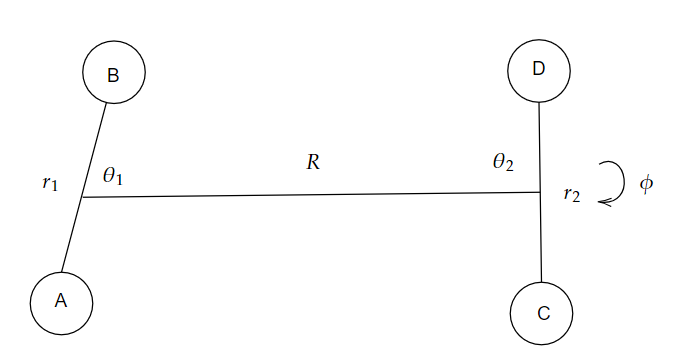
\includegraphics[scale=0.5]{2.png}
			\caption{Jacobi coordinates}
			\label{Figure2}
		\end{figure}
	\end{frame}
	\begin{frame}{Hamiltonian and Basis}
		The Hamiltonian can be written as
		\begin{align}
			H&=-\dfrac{\hbar^2}{2\mu_R}\nabla^2_R-\dfrac{\hbar^2}{2\mu_1}\nabla^2_{r_1}-\dfrac{\hbar^2}{2\mu_2}\nabla^2_{r_2}+V(\mathbf{R},\mathbf{r_1},\mathbf{r_2})\nonumber\\
			&=-\dfrac{\hbar^2}{2\mu_R}\dfrac{1}{R}\dfrac{\partial^2}{\partial R^2}R+\dfrac{\mathbf{L}^2}{2\mu_RR^2}-\dfrac{\hbar^2}{2\mu_1}\dfrac{1}{r_1}\dfrac{\partial^2}{\partial r_1^2}r_1+\dfrac{\mathbf{j_1}^2}{2\mu_1r_1^2}\nonumber\\
			&\quad-\dfrac{\hbar^2}{2\mu_2}\dfrac{1}{r_2}\dfrac{\partial^2}{\partial r_2^2}r_2+\dfrac{\mathbf{j_2}^2}{2\mu_2r_2^2}+V(\mathbf{R},\mathbf{r_1},\mathbf{r_2})
		\end{align}
		Now we have three angular momentum operators $(\mathbf{L},\mathbf{j_1},\mathbf{j_2})$ that are coupled to form the total angular momentum $\mathbf{J}$ which is conserved. 
	\end{frame}
	\begin{frame}{Hamiltonian and Basis}
		The method of choosing suitable basis sets to expand the wavefunction is essentially similar to that of triatomic systems. For example, we can expand the wavefunction as
		\begin{equation}
			\psi^{JM\epsilon}(\mathbf{R},\mathbf{r_1},\mathbf{r_2},t)=\sum\limits_{n\nu jK}C_{n\nu jK}\dfrac{u_n(R)}{R}\dfrac{\phi_\nu(r_1,r_2)}{r_1r_2}\mathcal{Y}^{JMp}_{j_{12}K}(\hat{\mathbf{R}},\hat{\mathbf{r_1}},\hat{\mathbf{r_2}})
		\end{equation}
		Here we have used the composite indexes $\nu$ and $j$ to denote collections of quantum numbers, i.e., $\nu=(\nu_1\nu_2)$ and $j=(j_1,j_2,j_{12})$ in order to simplify notation. The double vibrational basis $\phi_\nu(r_1,r_2)$ is defined as
		\begin{equation}
			\phi_\nu(r_1,r_2)=\phi_{\nu_1}(r_1)\phi_{\nu_2}(r_2)
		\end{equation}
		and $\mathcal{Y}^{JMp}_{j_{12}K}$ is the parity-adapted BF angular momentum basis function.
	\end{frame}
	\begin{frame}{Hamiltonian and Basis}
		It can be shown that the operation of the parity operator on the nonparity-adapted BF angular momentum basis yields the result
		\begin{equation}
			\hat{p}\mathcal{Y}^{JMp}_{j_{12}K}=(-1)^{j_1+j_2+j_{12}+J}\mathcal{Y}^{JMp}_{j_{12}-K}
		\end{equation}
		Thus we can define $\mathcal{Y}^{JMp}_{j_{12}K}$ by
		\begin{equation}
			\mathcal{Y}^{JMp}_{j_{12}K}(\hat{\mathbf{R}},\hat{\mathbf{r_1}},\hat{\mathbf{r_2}})=\dfrac{1}{\sqrt{2(1+\delta_{K0})}}\left[ \mathcal{Y}^{JMp}_{j_{12}K}+(-1)^{P+j_1+j_2+j_{12}}\mathcal{Y}^{JMp}_{j_{12}-K}\right] 
		\end{equation}
		where $P$ is the total parity.
	\end{frame}
	\begin{frame}{Hamiltonian and Basis}
		The BF basis
		\begin{equation}
			\mathcal{Y}^{JMp}_{j_{12}K}(\hat{\mathbf{R}},\hat{\mathbf{r_1}},\hat{\mathbf{r_2}})=\widetilde{D}^J_{KM}\mathcal{Y}^{j_{12}K}_{j_1j_2}
		\end{equation}
		where the normalization rotation matrix and Euler angles remain the same as for triatomics. The BF internal angular momentum function $\mathcal{Y}^{j_{12}K}_{j_1j_2}$ is defined as
		\begin{align}
			\mathcal{Y}^{j_{12}K}_{j_1j_2}(\theta_1,\theta_2,\phi)=&\sqrt{2\pi}\sum\limits_{m_1}\langle j_1m_1j_2K-m_1|j_{12}K\rangle\nonumber\\
			&\times\mathrm{Y}_{j_1m_1}(\theta_1,0)\mathrm{Y}_{j_2K-m_1}(\theta_2,\phi)
		\end{align}
		where $\mathrm{Y}_{jm}$ are spherical harmonics and $\phi_{12}$ is the out-of-plane torsional angles.
	\end{frame}
	\begin{frame}{Hamiltonian and Basis}
		The kinetic energy matrices are simple to evaluate and the treatment is not repeated here. The potential matrix in the angular basis for fixed radial coordinates $(R,r_1,r_2)$ can be calculated similarly to the case for triatomic molecules
		\begin{align}
			V^{JK_{jj^\prime}}(R,r_1,r_2)&=\langle JMjK|V|JMj^\prime K^\prime\rangle\nonumber\\
			&=\sum\limits_{m_1,m_1^\prime}\langle j_1m_1j_2K-m_1|j_{12}K\rangle\langle j_1^\prime m_1^\prime j_2^\prime K-m_1^\prime|j_{12}^\prime K\rangle\nonumber\\
			&\quad\times \int_0^\pi \mathrm{sin}\theta_1\mathrm{d}\theta_1\int_0^\pi \mathrm{sin}\theta_2\mathrm{d}\theta_2\mathrm{P}_{j_1m_1}(\theta_1)\mathrm{P}_{j_2K-m_1}(\theta_2)\nonumber\\
			&\quad\times V_{m_1,m_1^\prime}(R,r_1,r_2,\theta_1,\theta_2)\mathrm{P}_{j_1^\prime m_1^\prime}(\theta_1)\mathrm{P}_{j_2^\prime K-m_1^\prime}(\theta_2)
		\end{align}
		where
		\begin{equation}
			V_{m_1,m_1^\prime}=\dfrac{1}{\pi}\int_0^\pi\mathrm{d}\phi\mathrm{cos}[(m_1-m_1^\prime)\phi]V(R,r_1,r_2,\theta_1,\theta_2,\phi)
		\end{equation}
	\end{frame}
	\begin{frame}{Hamiltonian and Basis}
		The matrix element of the centrifugal potential can be calculated by a formula similar to that for triatomic molecules
		\begin{align}
			V_{K,K^\prime}^{cJj}&=\dfrac{\hbar^2}{2\mu R^2}\langle JMjK|(\mathbf{J-j_{12}})^2|JMj^\prime K^\prime\rangle\nonumber\\
			&=\dfrac{\hbar^2}{2\mu R^2}\delta_{jj^\prime}W_{KK^\prime}^{Jj_{12}}
		\end{align}
		where $W_{KK^\prime}^{Jj_{12}}$ is defined in \eqref{W} with the replacement of $j$ by $j_{12}$
	\end{frame}
	\begin{frame}{Hamiltonian and Basis}
		The full Hamiltonian matrix can now be constructed from separate pieces and has the following form
		\begin{align}
			H^J_{n\nu jK,n^\prime\nu^\prime j^\prime K^\prime}&=\langle JMn\nu jK|H|JMn^\prime \nu^\prime j^\prime K^\prime\rangle\nonumber\\
			&=\left[ \langle u_n|T_R|u_n^\prime\rangle\delta_{\nu\nu^\prime}+\langle \phi_\nu|T_{r_1}+T_{r_2}+\dfrac{\hbar^2}{2\mu_1r_1^2}j_1(j_1+1)\right.\nonumber\\
			&\left.\quad+\dfrac{\hbar^2}{2\mu_{r_2}r_2^2}j_2(j_2+1)|\phi_{\nu^\prime}\rangle\delta_{nn^\prime}\right] \delta_{jj^\prime}\delta_{KK^\prime}\nonumber\\
			&\quad+V^{JK}_{n\nu j,n^\prime\nu^\prime j^\prime}\delta_{KK^\prime}+V^{cJj}_{nK,n^\prime K^\prime}\delta_{\nu\nu^\prime}\delta_{jj^\prime}
		\end{align}
		where $T_R, T_{r_1}$ and $T_{r_2}$ are the kinetic energy operators corresponding to the $R, r_1$ and $r_2$ radial coordinates in the Hamilonian.
	\end{frame}
	\begin{frame}{Hamiltonian and Basis}
		Here the full potential matrices are calculated from the angular part by
		\begin{equation}
			V^{JK}_{n\nu j,n^\prime\nu^\prime j^\prime}=\langle u_n\phi_\nu|V^{JK}_{j,j^\prime}|\phi_{\nu^\prime}u_{n^\prime}\rangle
		\end{equation}
		and
		\begin{equation}
			V^{cJj}_{nK,n^\prime K^\prime}=\langle u_n|V^{cJj}_{K,K^\prime}|u_{n^\prime}\rangle
		\end{equation}
		The bound state problem is then solved by diagonalizing the Hamiltonian matrix, provided that the size of the matrix is not prohibitively large.
	\end{frame}
	\begin{frame}{Symmetry for Two Identiacl Monomers}
		if AB and CD are identical momomers as in $(\mathrm{HF})_2$, the rovibrational eigenfunctions $X^{JMp}_{\nu jK}=\mathcal{Y}^{JMp}_{jK}\phi_\nu$ should be properly symmetrized. The symmetrized rovibrational basis can be written as
		\begin{equation}
			X^{\pm JMp}_{\nu jK}=\left[ 2\left( 1\pm\langle X^{JMp}_{\nu jK}|\hat{p}_{ex}|X^{JMp}_{\nu jK}\rangle\right) \right] ^{-1/2}\left[ X^{JMp}_{\nu jK}\pm\hat{p}_{ex}X^{JMp}_{\nu jK}\right] 
		\end{equation}
		where $\hat{p}_{ex}$ is the exchange operator that changes the coordinates $(\mathbf{r_1},\mathbf{r_2},\mathbf{R})\rightarrow(\mathbf{r_2},\mathbf{r_1},-\mathbf{R})$. It can shown that
		\begin{equation}
			\hat{p}_{ex}X^{JMp}_{\nu jK}=(-1)^{p+j_{12}}X^{JMp}_{\tilde{\nu} \tilde{\jmath}K}
		\end{equation}
		where $\tilde{\nu}$ and $\tilde{\jmath}$ denote transposed indexes $(j_2,j_1,j_{12})$ and $(\nu_2,\nu_1)$.
	\end{frame}
	\begin{frame}{Symmetry for Two Identiacl Monomers}
		Thus the symmetrized basis is
		\begin{equation}
			X^{\pm JMp}_{\nu jK}=\Delta_{\nu j,\tilde{\nu}\tilde{\jmath}}\left[ \mathcal{Y}^{JMp}_{jK}\Phi_\nu\pm(-1)^{j_{12}+p}\mathcal{Y}^{JMp}_{\tilde{\jmath}K}\Phi_{\tilde{\nu}}\right] 
		\end{equation}
		where the normalized constant is given by
		\begin{equation}
			\Delta_{\nu j,\tilde{\nu}\tilde{\jmath}}=[2(1+\delta_{\nu\tilde{\nu}}\delta_{j\tilde{\jmath}})]^{-1/2}=[2(1+\delta_{\nu_1\nu_2}\delta_{j_1j_2})]^{-1/2}
		\end{equation}
		Here we note that quantum numbers $\nu$ and $j$ are restricted by the requirement of $\nu_1\geqslant\nu_2$ and $j_1\geqslant j_2$ for $\nu_1=\nu_2$. Note that for $\nu_1=\nu_2$ and $j_1=j_2$, the allowed $j_{12}$ quantum numbers must satisfy the condition $p_{ex}(-1)^{j_{12}+p}=1$.
	\end{frame}
	\begin{frame}{Symmetry for Two Identiacl Monomers}
		The potential matrix elements in the symmetrized basis representation $X^{\pm JMp}_{\nu jK}$ can be written explicitly in terms of unsymmetrized functions
		\begin{align}
			\langle X^{\pm JMp}_{\nu jK}|V|X^{\pm JMp}_{\nu^\prime j^\prime K^\prime}\rangle=&2\Delta_{\nu j,\tilde{\nu}\tilde{\jmath}}\Delta_{\nu^\prime j^\prime,\tilde{\nu}^\prime\tilde{\jmath}^\prime}\delta_{KK^\prime}\left[ \mathcal{Y}^{JMp}_{jK}|V_{\nu\nu^\prime}|\mathcal{Y}^{JMp}_{j^\prime K}\rangle\right.\nonumber\\
			&\left.\pm(-1)^{j_{12}+p}\langle\mathcal{Y}^{JM}_{\tilde{\jmath}K}|V_{\tilde{\nu}\nu^\prime}|\mathcal{Y}^{JMp}_{j^\prime K}\rangle\right] 
		\end{align}
		where
		\begin{equation}
			V_{\nu\nu^\prime}=\langle\phi_\nu|V|\phi_{\nu^\prime}\rangle
		\end{equation}
		and 
		\begin{equation}
			V_{\tilde{\nu}\nu^\prime}=\langle\phi_{\tilde{\nu}}|V|\phi_{\nu^\prime}\rangle
		\end{equation}
		The centrifugal potential in the symmetrized basis representation is given by
		\begin{align}
			\langle &X^{\pm JMp}_{\nu jK}|V_c|X^{\pm JMp}_{\nu^\prime j^\prime K^\prime}\rangle =\nonumber\\
			&\Delta_{\nu j,\tilde{\nu}\tilde{\jmath}}\Delta_{\nu^\prime j^\prime,\tilde{\nu}^\prime\tilde{\jmath}^\prime}\dfrac{\hbar^2}{\mu R^2}\left[ \delta_{\nu\nu^\prime}\delta_{jj^\prime}\pm(-1)^{j_{12}+p}\delta_{\tilde{\nu}\nu^\prime}\delta_{\tilde{\jmath}j^\prime}\right] W^{Jj_{12}}_{K,K^\prime}
		\end{align}
	\end{frame}
\end{document} 
